%! Author = adam
%! Date = 28.02.21


\chapter{Ion Range and Impact on Solid State Computer Design}\label{ch:ion-range-and-impact-on-solid-state-computer-design}
In this chapter we will examine the following topics:
\begin{myitemize}
	\item Ion Range
	\item Displacements/Damage
	\item SRIM Simulation
	\item Channeling
\end{myitemize}

We want to build the connection of the previous chapter to the ion range, i.e., the range or depth in which the ion enters the sample.
The Figure~\ref{fig:ionstop} gives a visualization of the depth of which the ion goes in the solid.
For high energy particles or low mass ions, the electronic stopping dominates, and the low energy nuclear dominates.
For heavy ions (lead for example), there will always be a domination of the electronic stopping, i.e., the range depends heavily on the mass and energy of the ion.
Ion range has a great practical importance for radiation therapy, as we will see later when it comes to Bragg Peaks.

\section{Ion Range}\label{sec:ion-range}
We first have to define a bit of terminology in which we can discuss the depth of the ion entering into the sample.
Imagine a surface plane of a material in a coordinate system of your choosing.
An ion then impacts the beam with a certain angle $\alpha$ relative to the normal of the surface of the plane.
Due to elastic collision, we will not have a straight path through the sample of the ion, but rather a jagged path.
There are different definitions of the ion range, one most discussed is called the \textit{projected range} $R_p$.
This is the projected distance in which the ion would go if it was not deflected.
The \textit{transversal projected range}, $R_p^t$, is the length between the real end point of the ion normal to the projected range.
The direct distance between the point of rest and the point of incident is the \textit{radial range}, $R_r$.
Imagine now we take the point of rest, and we take a projection of this point to the surface plane.
The distance from this point on the plane to the incident point is called the spread, $R_s$.
Since we have a certain angle of incident, the radial range is not the same as the penetration depth of the ion, therefore the depth $x_s$ is normal to the surface plane.
Definitions of the various terms are given below, where the point $(x_s, y_s, z_s)$ is the point in which the ion stops (in cartesian coordinates) beneath the sample surface plane.

\begin{gather*}
    R_s = \left( y_s^2 + z_s^2 \right)^{1/2}\\
    R_r = \left( x_s^2 + y_s^2 + z_s^2 \right)^{1/2}\\
    R_p^t = \left[ \left( x_s \sin(\alpha) - y_s\cos(\alpha) \right)^2 + z_s^2 \right] ^{1/2}\\
    R_p = \left[ R_r^2 + R_p^{t2}\right] ^{1/2}\\
\end{gather*}
If $\alpha = 0$, $R_p = x_s$, and $R_s = R_p^t$.
\subsection{Distribution}\label{subsec:distribution}
Discussed above is the case for a single ion, but since we use ion beams normally, this will result in some sort of distribution since stopping is a random and thus stochastic process for each individual ion.
The total ion path length will then be different for each ion, i.e., statistically broad distributions of ion penetration depth.
This range distribution, also called the \textit{straggling}, can be quantified using the density of particles $N$ given the depth within the sample $x$, $\rightarrow N(X)$:
\begin{equation}
	N(x) = \frac{\Phi_i}{\Delta R_p \sqrt{2\pi}} exp \left[ -\frac{1}{2} \left( \frac{x - R_p^2}{\Delta R_p}\right) ^2\right]
	\label{eq:struggle}
\end{equation}
where $\Delta R_p$ is the projected range straggling, and $R_p$ is the projected range (mean depth). $\Phi_i$ is called the fluency, and is defined,  $\Phi_i =  \int_{-\infty}^\infty N(x)dx$.
From~\ref{eq:struggle}, we can see that $N(R_p) = N_p = \frac{\Phi_i}{\Delta R_p 2\phi}$
One would end up with a gaussian distribution for $N(x)$, with maximum at $x = R_p$, with the FWHM being equal to $2 \Delta R_p$
Normally, for 100 kV Boron implanted into Silicon, the mean penetration depth will be about 380 nm, but with straggling of mostly 90 nm.
Usually, one would use $1/$cm$^2$ for a unit of fluency, therefore straggling will also have units of cm.
$N_p$, the number of ions at mean penetration depth will be in units of atoms per cm$^3$.
For all other quantities related to the range, i.e., depth or longitudinal range, can also be distributed using this method.

\subsection{Bragg Peak}\label{subsec:bragg-peak}
We see that the energy loss per unit distance increases as the particle slows down.
The curve describing this fact is the Bragg curve.
Shortly before the end, the energy los passes through a maximum, the \textbf{Bragg Peak}, then drops to zero.
More is discussed in~\ref{fig:bragg}.
This is used in cancer treatment.
This is fantastic, since we know that for high energy, there will be low energy deposition at the beginning of the depth, followed by an extremely high increase in interaction and nuclear stopping at the end.
\begin{figure}
	\centering
	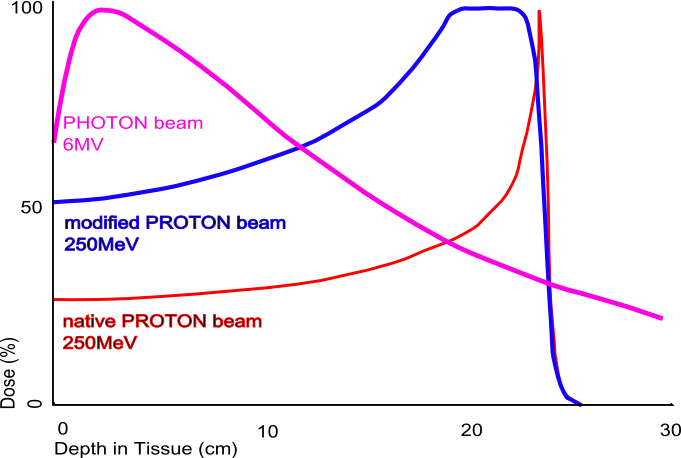
\includegraphics[scale=0.4]{BraggPeak}
	\caption{Here we have various proton beams, with increasing energy, as a function of depth within the tissue. For a native Proton beam, we have a low loss of energy due to the electronic stopping, and therefore an increase in interactions, and finally a peak in the energy interactions at a certain position, called the Bragg peak.}
	\label{fig:bragg}
\end{figure}


\section{Displacement and Damage}\label{sec:displacement-and-damage}
Not only is the path of the ion important, but also the displacement of atoms within the sample due to the ion important.
The type of motion exhibited by the atoms is modeled by a phenomena called cascade.
There are some nice videos on youtube (\href{https://www.youtube.com/watch?v=HNFwXnGmie4}{example}), where we see that the ion collides with an atom, called the \textit{primary knock on atom}, which then goes on to cause a cascade of other collisions with other atoms within the sample.
The displacement threshold, or energy, in which a collision would occur is denoted by $E_d$, this is the minimum energy that an ion (or atom in the case of it being already displaced and is moving to displace other atoms) must have in order to displace an atom from its lattice site.
We consider two temperature ranges, one below the threshold and one above.
For $T < E_d$, there is a vibration as the atom that was struck by the ion quickly shares its energy with the nearest neighbor atoms, i.e., a local heat source.
For $T > E_d$, it is a displaced atom, i.e., the simplest case, and the atom is deflected just like how an ion would be deflected, leading to vacancy-interstitial pairs (Frenkel pair) in the atomic structure due to the displaced atom.
But, we can only really define an average $ \langle E_d \rangle $, since $E_d$ depends on direction.
For example, the $ \langle E_d \rangle $ for Silicon is around 16eV, and for Aluminum 43 eV.

\subsection{Kinchin-Pease Model}\label{subsec:kinchin-pease-model}
Let's assume we have the energy of the primary knock on (PKA) atom, which has energy $E_\nu >> E_d$, so the PKA will have many more recoil atoms and displacements following from it.
This displaced atoms can in turn displace additional atoms.
At the end we will end up with many collisions and displacement events which occur in proximity with each other.
Therefore we can introduce the \textit{displacement damage function}, $\langle N_d (E) \rangle $, which of course depends on the energy of the PKA.
This is just the average number of displaced atoms in a cascade produced by a PKA.
The simplest model for this is the Kinchin-Pease model, based on a hard sphere model, where the nuclei of the atoms are assumed to be hard spheres.
The KP model has the following assumptions, which turn out to be good enough for approximations.

\begin{myitemize}
	\item Collision between like atoms,  i.e., $M_1 = M_2$
	\item Hard-sphere cross section, i.e., $P(E,T)dT \approx \frac{dT}{E}$
	\item Cascade of two body collisions, (binary collision approximation)
	\item Elastic nuclear collisions
	\item $E_d$ neglected in energy balance of elastic collision
	\item No crystal structure
	\item $T < E_d \rightarrow $ no displacement
	\item $E < E_d$ for a knock-on atom $\rightarrow $ no further contribution to cascade
	\item atoms receiving $E_d< E < 2E_d$ are displaced but can not themselves further increase the total number of displacements
\end{myitemize}
In the Kinchin-Pease model the number of point defects generated by an implanted ion is derived analytically from the energy that is transferred from an ion to an atom of the target material.
It is assumed that the number of point defects generated by a primary recoil is proportional to the energy transfered from the ion to the primary recoil.
A primary recoil is a recoil generated by the collision of an implanted ion with a target atom, while secondary recoils are generated by recoils.
Using this we can approximate the number of Frenkel pairs $N_d$ generated by a PKA atom.
$$ \langle N_d (E_\nu) \rangle = \begin{cases}
			 0 & E_\nu < E_d \\
			 1 &  E_d < E_\nu < 2E_d \\
			 \frac{E_\nu}{2E_d} & 2E_d < E_{\nu} < E_c \\
			 \frac{E_c}{2E_d} & E_{\nu} > E_c
\end{cases} $$

Here, we detail the above relations.
For the first case, it is obvious that there will be 0 point defects for an energy less than the displacement energy.
For the second relation, we will have a total of 1 displacement for energies between $E_d $ and $2 E_d$, from which there are two possibilities.
The PKA can cause a collision with another atom, which the transmitted energy could be $E_d < T < 2E_d$, and the lattice atom will be displaced.
The initial PKA is then left with an energy less than the displacement energy, therefore the initial PKA is left with $E_\nu < E_d$, so no stable Frenkel pair, and the PKA falls into the vacant site left by the displaced atom.
This is called a \textit{replacement collision}, and is more probable than a permanent replacement.
For a transmitted energy $T \rightarrow T < E_d \Rightarrow$ lattice atom will \textunderscore{not} be replaced.
The primary PKA atom is left with insufficient  $E_\nu$ for other displacement.
In both cases we are moving one atom which has less energy than the initial PKA.
Therefore with PKA with energy between $E_d$ and $2E_d$ we will leave with only one displaced atom.
For mono-atomic samples, these two cases make really no difference, but with multi-atomic samples we can change which atom is at which lattice site.

Now we can ask what happens for $E_\nu > 2E_d$.
We have to calculate the average recoil energy $\langle T \rangle $ produced by a PKA with energy $E_\nu$.
$$ \langle T =  \rangle \int_0^{T_M} T P(E,T) dT = \frac{1}{T_M} \int_0^{T_M} TdT = \frac{E_\nu}{2} $$
The $P(E,T)$ term comes from the hard sphere cross section assumption, and is the probability of a certain transfer energy to occur, and $PdT = dT / E$.
The maximum transfered energy possible $T_M$ is really just the energy of the atom $E_\nu$.
Finally, this leads us to be able to calculate the average number of displacements produced by a mean recoil energy, $\frac{\langle T \rangle}{E_d} = \frac{E_\nu}{2E_d}$

But for high energies $T$, we will have some diversion, so we define the critical energy $E_c$ to take into account the electronic losses of PKA.
It is just the mass number of the element times 1 keV, i.e., $E_c = M_2$keV. The typical value of $E_c $ for copper is $62$ keV.
For PKA's with $E > E_c$, the distribution can be written as a constant value:
$$\langle N_d (E_\nu) \rangle  = \frac{E_c}{2E_d}$$


\section{Let's Build a Solid State Quantum Computer}\label{sec:let's-build-a-solid-state-quantum-computer}
A very short introduction to the criteria for a SSQC. We need to fulfill these criteria in order to build one, and were defined by Divencenzo.
Initially there were just five conditions, but if we want to do quantum communications we need the last two.
\begin{enumerate}
	\item A \textbf{scalable} physical system with well characterized qubit
	\item The ability to \textbf{initialize} the state of the qubits to a simple fiducial state
	\item Long relevant \textbf{decoherence} times
	\item A "universal" set of quantum \textbf{gates}
	\item A qubit-specific \textbf{measurement} capability
	\item The ability to \textbf{interconvert} stationary and flying qubits
	\item The ability to faithfully \textbf{transmit} flying qubits between specified locations
\end{enumerate}
In the context of ion implantation, there are two things that are important, as the technique of implantation will directly correlated scalability and decoherence.
Scalability means that we will not only have to be able to produce one qubit, but rather multiple qubits.
Decoherence time should be very long so that we can actually use these qubits.
The implantation needs to be deterministic, i.e., if we want to implant an ion in a sample, we need to be sure that we can do this with however many ions we want to put there.
Some questions to consider before reading on:
\begin{myitemize}
	\item What could be the bottleneck of ion beam techniques and what are the advantages for building a solid-state quantum computer?
	\item What are the challenges?
\end{myitemize}


\section{Summary}\label{sec:summary5}

\begin{myitemize}
	\item With ion beams, the scattering of the ions within the sample is a stochastic process, and can be modeled using distribution functions
	\item Straggling is the distribution of these ions due to the stochastic processes, and has a major impact in the building of a quantum computer in the solid state.
	\item Bragg peaks define where in the penetration depth a high increase in transmitted energy will occur
	\item KP model is a simple set of assumptions to help describe how atoms will interact with each other depending on their energies after being struck by a penetrating ion or atoms that were first struck by the ion (PKA's)
	\item Ion implantation physics like straggling have a great influence on theoretical quantum computers, as if we wanted to create qubits we would find restrictions like $E \leq 10 keV$ to not allow for straggling to take over spatial resolution.
\end{myitemize}

